\documentclass[xcolor=dvipsnames]{beamer}

% font setup
\usepackage{libertine}
\renewcommand*\familydefault{\sfdefault}    % Linux Libertine = default sans serif
\usepackage{inconsolata}                    % Inconsolata = monospaced
\usepackage[utf8]{inputenc}
\usepackage[T1]{fontenc}
\usepackage{tikz}
\usetikzlibrary{positioning}

\usepackage{algorithm}
\usepackage{algpseudocode}
\makeatletter
\renewcommand{\ALG@name}{Algoritm}
\makeatother
\algrenewcommand\algorithmicprocedure{\textbf{procedură}}
\algrenewcommand\algorithmicend{\textbf{final}}

% Graphics and other packages
\usepackage[romanian]{babel}
\usepackage{graphicx}
\addto\captionsromanian{\renewcommand{\figurename}{Ilustrație}}
\usepackage{caption}
\usepackage{subcaption}
\usepackage[style=german]{csquotes}

% Custom macros
\newcommand{\bloc}[3]{\begin{bl}<#1->{{\large\color{Gray}{\hrulefill}}\\ \color{bleumarin}{\large \emph{#2}}}\\ \vspace*{-2mm}{\color{Gray}{\hrulefill}}\\ #3 \end{bl}} 
\newcommand{\fr}[1]{\frame{#1}}
\newcommand{\ft}[1]{\frametitle{\color{bleumarin}{\hfill #1 \hfill}}}
\newcommand{\lin}[3]{\uncover<#1->{\alert<#1>{#2}}{\vspace*{#3 ex}}}
\newcommand{\ite}[2]{\uncover<#1->{\alert<#1>{\item #2}}}
\newcommand{\vs}[1]{\vspace*{#1 ex}}
\definecolor{bleumarin}{RGB}{30,30,150} 
\definecolor{firebrick}{RGB}{178,34,34}

% Theme setup
\useoutertheme{shadow} 
\usetheme{CambridgeUS} 
\usecolortheme[named=bleumarin]{structure} 
\useoutertheme[compress]{smoothbars}

% Theme finetuning
\setbeamertemplate{items}[ball]
\setbeamertemplate{blocks}[rounded][shadow=true]
\setbeamertemplate{navigation symbols}{}
\setbeamertemplate{headline}{}  


%%%%%%%%%%%%%%%%%%%%%%%%%%%%%%%%%%%%%%%%%%%%%%%%%%%%%%%%%%%%%%%%%%%%%% 
% TITLE PAGE
\title{Numărul de puncte de pe curbe eliptice}
\author[Adrian Manea]{Adrian Manea \\ {\scriptsize GitHub \texttt{@adimanea/sla/3-criptav/\{current,beamer\}}}}
\institute{510, SLA}

\date{}

\begin{document}

\maketitle

% SLIDES START HERE
%%%%%%%%%%%%%%%%%%%%%%%%%%%%%%%%%%%%%%%%%%%%%%%%%%%%%%%%%%%%%%%%%%%%%% 
\fr{
  \ft{Ideea}

  \lin{1}{Curbe eliptice = obiecte geometrice cu structură algebrică;}{3}

  \lin{2}{Pot fi studiate ca ecuații diofantice (peste $ \mathbb{Q} $);}{3}

  \lin{3}{Structura algebrică permite operații între soluții;}{3}

  \lin{4}{Soluțiile se găsesc greu $ \Rightarrow $ operațiile cu ele sînt
    destul de sigure criptografic.}{3}
}

\fr{
  \ft{Curbe eliptice}

  \lin{1}{Forma simplă (Weierstrass): $ y^2 = x^3 + ax + b $;}{3}

  \lin{2}{
    \begin{figure}[!htbp]
      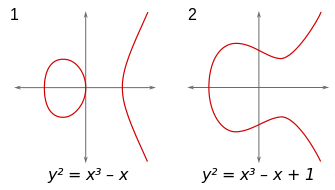
\includegraphics[scale=0.6]{fig/ec.png}
      \caption{Curbe eliptice [Wikipedia]}
    \end{figure}
  }{2}
}

\fr{
  \ft{Puncte pe curbe eliptice}

  \lin{1}{\textbf{Exemplu:} $ E : y^2 = x^3 + 17 $.}{3}

  \lin{2}{$ P_1(-2, 3), P_2(-1, 4), P_3(2, 5), P_4(4, 9), P_5(8, 23) \in E $.}{3}

  \lin{3}{Are loc $ P_5 = -2 \cdot P_1, P_4 = P_1 - P_3 $, cu operația următoare: }{3}
}

\fr{
  \ft{Grupul definit de o curbă eliptică}

  \begin{figure}[!htbp]
    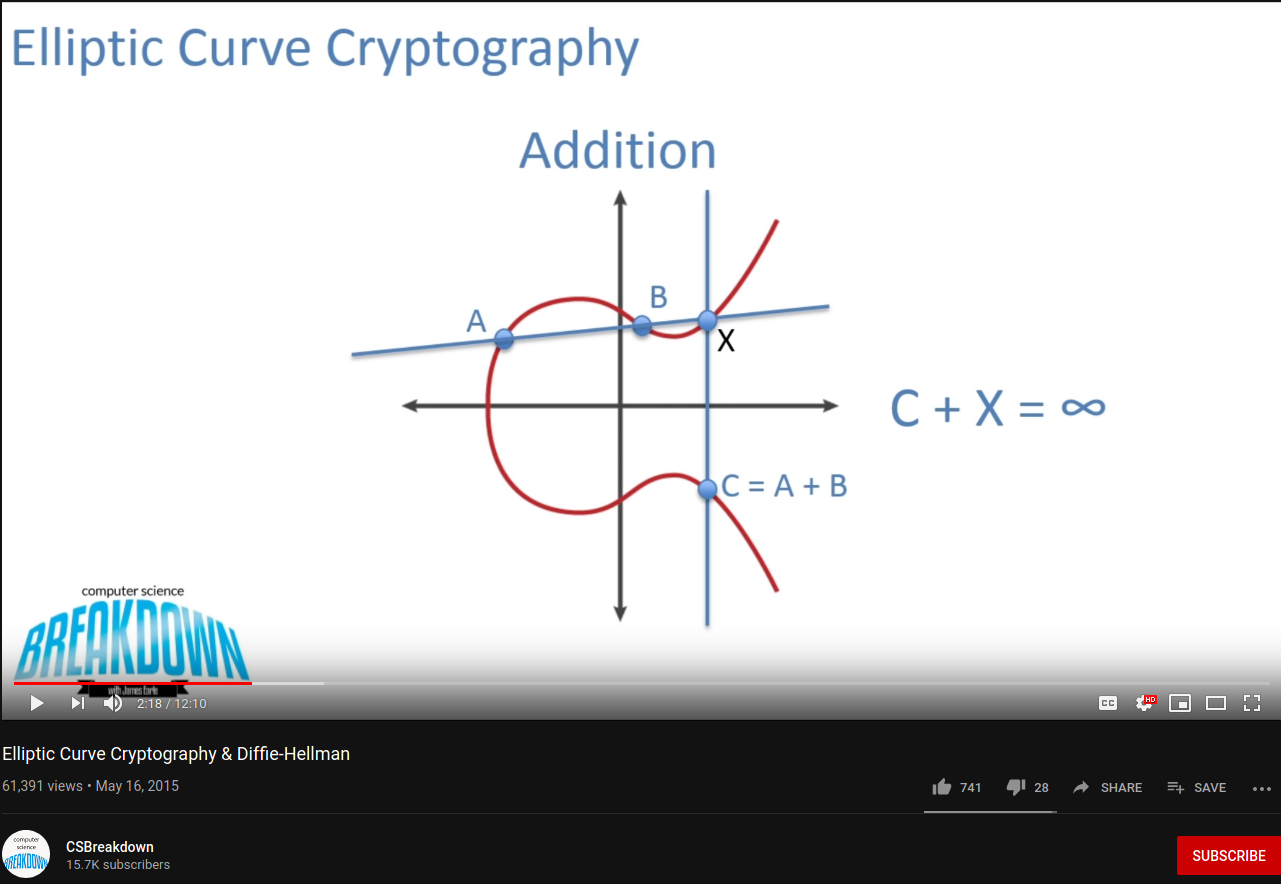
\includegraphics[scale=0.22]{fig/ec-yt.png}
    \caption{Adunarea punctelor de pe o curbă eliptică [YT \texttt{@CSBreakdown}]}
  \end{figure}
}

\fr{
  \ft{Numărul de puncte ($\#E(K)$)}

  \lin{1}{Depinde de corpul $ K $ peste care este definită curba $ E $!}{0}

  \lin{2}{Exemplu simplu: peste $ \mathbb{F}_5, E: y^2 = x^3 + x + 1 $:}{0}

  \lin{3}{
    \begin{center}
      \begin{tabular}{|c|c|c|c|c|}
        \hline
        $ x $ & $ x^2 $ & $ x^3 + x + 1 $ & $ y $ & Puncte \\
        \hline
        0 & 0 & 1 & 1, 4 & $ (0, 1), (0, 4) $ \\
        1 & 1 & 3 & $ \nexists $ & $ \nexists $ \\
        2 & 4 & 1 & 1, 4 & $ (2, 1), (2, 4) $ \\
        3 & 4 & 1 & 1, 4 & $ (3, 1), (3, 4) $ \\
        4 & 1 & 4 & 2, 3 & $ (4, 2), (4, 3) $ \\
        \hline
      \end{tabular}
    \end{center}
  }{2}

  \lin{4}{Rezultă $ \#E(\mathbb{F}_5) = 9 $, calculat manual în $ O(5) $ pași.}{0}
}


\fr{
  \ft{Optimizări}

  \lin{1}{În general, naiv avem $ \# E(\mathbb{F}_q) \leq 2q + 1 $.}{0}

  \begin{itemize}
    \ite{1}{\textbf{Teorema lui Hasse (1924 [E.\ Artin] -- 1933)} (\cite{soe,sil09}):
      \[
        \left| \# E(\mathbb{F}_q) - q - 1 \right| \leq 2 \sqrt{q};
      \]}
    \ite{2}{\textbf{Baby Step, Giant Step} (pentru log discret) $ \Rightarrow 4 \sqrt[4]{q} $;}
    \ite{3}{\textbf{Algoritmul Schoof} (\cite{sil09}) $ \Rightarrow O(\log^8 q) $ = POLY;}
  \end{itemize}
}

\fr{
  \ft{Observații și concluzii}

  \lin{1}{Pentru $ q \simeq 2^{256} $, Schoof lucrează cu numere pe 16 kB!}{5}

  \lin{2}{Continuare: Elkies, Atkin (cca.\ 1994) (\cite{galin}) $ \Rightarrow O(\log^6 q) $.}{5}

  \lin{3}{Folosește unele presupuneri euristice (incl.\ ipoteza lui Riemann).}{5}
}
%%%%%%%%%%%%%%%%%%%%%%%%%%%%%%%%%%%%%%%%%%%%%%%%%%%%%%%%%%%%%%%%%%%%%% 

% Bibliography
\fr{
  \ft{Bibliografie}
  \bibliography{pce-prez.bib}
  \bibliographystyle{apalike}
}
\end{document}

